% !TEX root = main.tex
\chapter{Design and simulation of the addressing setup}
The purpose of this thesis work was to develop a single-ion-addressed laser system for generating single photons and for single ion-qubit control. In this chapter we discuss the design and the implementation of such a system. The design is a crucial part of the work, since there are several requirements that have to be met in order to achieve the desired functionality. In the first section, the requirements are presented together with an overview of the design idea. In the setup an objective was already present, and the choice of an AOD was already made, in anticipation of my project. Hence, we discuss these components as given. The rest of the setup was simulated with the software Zemax, which was used to find the optimal additional optical components and their placement.
\section{Addressing system overview and requirements}
\label{sec:addressing}
Single-ion addressing laser systems have already been developed and employed in experiments successfully in Innsbruck and elsewhere. The main idea is to focus a laser beam tighter than ion-ion separation and steer it between different ions on a few micro-second timescale. In Innsbruck, calcium ions have been addressed in this way, where the steering was achieved with an AOD \cite{addressing}; At Duke university, laser beams have also been steered with micro-electromechanical systems (MEMS) mirrors \cite{addressing3}. Another idea is to send a beam illuminating all the ions, but hiding those who are not addressed. This was done with Ytterbium atoms by means of a inhomogeneous magnetic field the transition frequencies were shifted shielding selected ions \cite{addressing2}. \par
Our choice was to implement the approach of Innsbruck with an AOD and improve it. A problem with the implementation of \cite{addressing} is limited addressing range as the beam clips on the edge of optics when working with strings of ten ions or more at typical confinement. Furthermore, their system is developed for 729 nm light, while our goal is use the 393 nm transition, this requires new simulations and different optics. Therefore, the new designed system aims to exploit the full capabilities of the AOD while maintaining a waist of a few microns or less. The shorter 393 nm wavelength offer us the chance for even tighter focuses than have previously been achieved at 729 nm with similar optics.
\begin{figure}
\centering
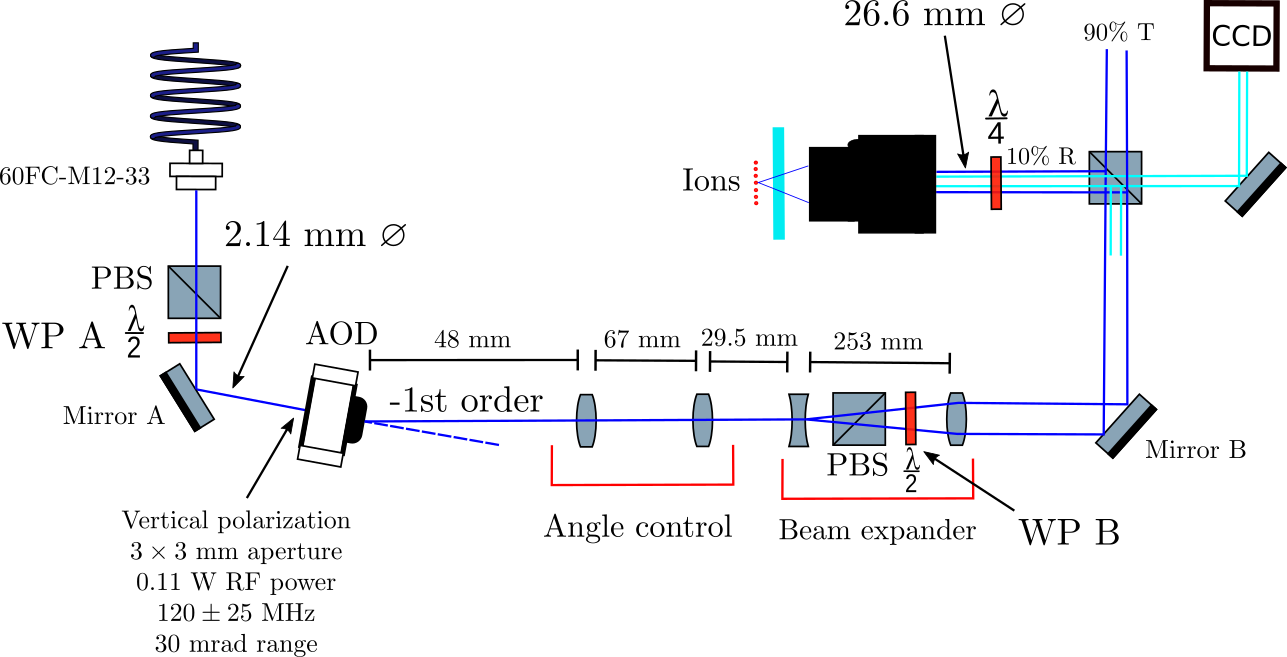
\includegraphics[width=\textwidth]{setup}
\caption{Final schematic of the 393 nm laser single-ion addressed optical setup. Light comes from a fiber, polarization is cleaned, and then sent thorough the AOD from Gooch \& Housego 4120-3. -1st order diffracted light is sent into a beam expander, where the beam is broadened before being focused by the objective. All lenses are from Thorlabs, models are from left to right: LA-1509, LA-1131, LC-4252, LA-1725; all of them are AR coated for 393 nm. Critical distances between lenses are in the figure, distance between the last lens and the first lens of the objective is 722 mm. The 90:10 Beam splitter is custom made by Laser Components GmbH. Diameters $\varnothing$ are expressed as $1/e^2$ of intensity. Between objective and ions there is a 6 mm thick glass of the viewport, as the objective is out of vacuum. $\lambda/2$ waveplates are labeled as WP A, and WP B for future reference. Light blue lines represents 397 nm scattered photons coming from the ions into the imaging setup.}
\label{addressingsetup}
\end{figure}
The addressing setup should be able to address single ions in a string in order to generate single photons out of single ions via the already discussed Raman process. Ion separations have been derived in Section \ref{ionstrings}. In the case of two $^{40}\text{Ca}^+$, the separation between the two ions is 5.6 $\mu$m for an axial center of mass frequency of 1 MHz. The setup must therefore be able to focus a laser beam down to 1-2 $\mu$m waist to minimize cross talk. As seen in Section \ref{sec_diffraction}, a tighter focus can obtained with a shorter wavelength, a bigger lens, or with a shorter focal length. The focusing lens, i.e. the objective, is shared with the imaging setup, and thus it is given, the focal length (66.8 mm) is therefore a constant in the problem, see Section \ref{sec:obj}. The wavelength is also a constant, as the Raman process happens at 393 nm. This gives only one possibility left to tighten the focus, i.e. by making the beam as broad as possible at the objective input surface.\par
Figure \ref{addressingsetup} presents the final layout of the addressing setup. Some key aspects are now discussed. Beam expansion is achieved with a Galilean telescope composed of two lenses: a concave lens for diverging a collimated beam and a convex lens for collimating the diverging beam. The combination of these two lenses takes a collimated beam and expands it to another approximately collimated beam with an expansion factor of 23.9\footnote{Since the beam is not collimated after the beam expander, the expansion factor has been calculated as the ratio of the incoming and outgoing beam diameters of the beam expander.}. This expansion part is one of the two essential parts of the addressing setup. The other part is related to the addressing spatial range. We want not only to focus the beam to a single ion, but also to move the beam as well, such that it focuses on a different ion. Therefore, there is a requirement also on the range that can be addressed. This depends on the number of ions and their spacing. We chose to aim to address many tens of ions, this requires the ability to move the focus along the ion string by 150-200 $\mu$m. Beam steering is possible with the use of an AOD, the detailed working principle of this device has been discussed in Section \ref{theory_AOD}. Basically, the angle of the output beam of the AOD changes as the driving frequency changes. However, the AOD must be placed far behind the objective to leave space for the beam expander, leading to the need to redirect the angular change of the AOD's output. This task is accomplished with a pair of converging lenses (Angle control in Figure \ref{addressingsetup}), which refocus the collimated beam into the beam expander, the beam then becomes wider, reaches the objective and is focused on the ion. The objective was not designed to focus incoming collimated blue light onto the ions, but rather to image 397 nm photons from the ions onto a camera 1.5 m away from the objective. Simulations showed that a slightly diverging 393 nm beam ($\sim 0.5^\circ$), incoming into the objective, will be focused onto the ions. As such, we set the telescope to expand the beam without collimating it, leaving it diverging, so that the objective can focus it at the right position.\par
The setup displayed in Figure \ref{addressingsetup} contains polarization optics. As discussed in Section \ref{sec:ramanprocess}, Zeeman transitions are polarization sensitive, thus polarization control is required. In order to control the polarization at the point of the ion a half-waveplate and a quarter-waveplate are inserted in the optical path. The position of the quarter-waveplate, right before the objective, means that it is unusually big (2 inches in diameter), but if placed before in the optical path, the mirror and the beam splitter could alter the polarization. The quarter wave plate is zeroth order and custom made by CeNing Optics, in order to have a greater polarization stability.\par
The choice of a 90:10 beam splitter (Figure \ref{addressingsetup}) to overlap the incoming 393 nm addressing laser with the outgoing 397 nm ion fluorescence for imaging is unusual: a more obvious choice would be to use a dichroic mirror. However, the light in the imaging path is 397 nm, very close to the 393 nm light of the addressing setup. This would have meant using a very narrow dichroic. Instead, we use a 90:10 beam splitter, where 90\% of the light is transmitted and only 10\% of the light is reflected. In this way, only 10\% of imaging light is lost, at cost of 90\% of addressing laser light, which is not such a problem as power from the laser is available. Furthermore, this light is focused so tightly that even a small amount of light can excite the ions. On the other end, it is not so straightforward to get more scattered light from the ions, so 397 nm light and the imaging setup must be as efficient as possible, with 10\% losses, ions states are still distinguishable on the camera without significantly extending the detection times required.

\section{Objective and AOD}
\label{sec:obj}
% \begin{figure}[H]
%      \centering
%      \begin{subfigure}[b]{0.4\textwidth}
%          \centering
%          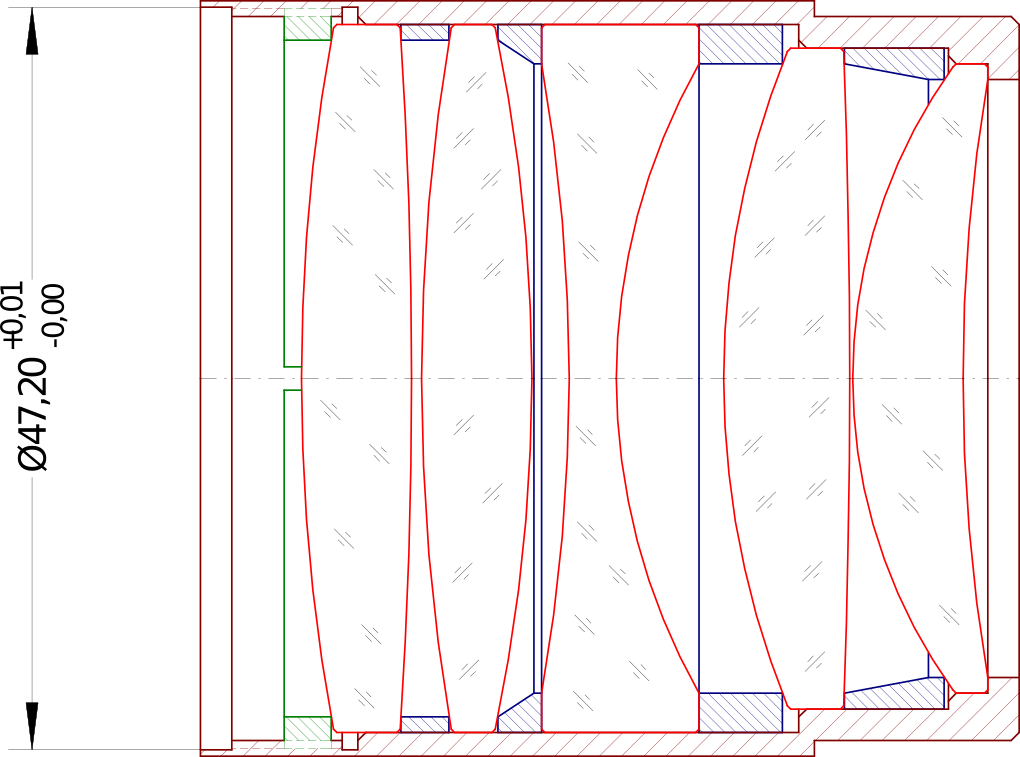
\includegraphics[width = \textwidth]{obj}
%           \caption{Section of the custom objective, red parts are the lenses, while the rest is the housing.}
%          \label{objsection}
%      \end{subfigure}
%      \hfill
%      \begin{subfigure}[b]{0.55\textwidth}
%          \centering
%          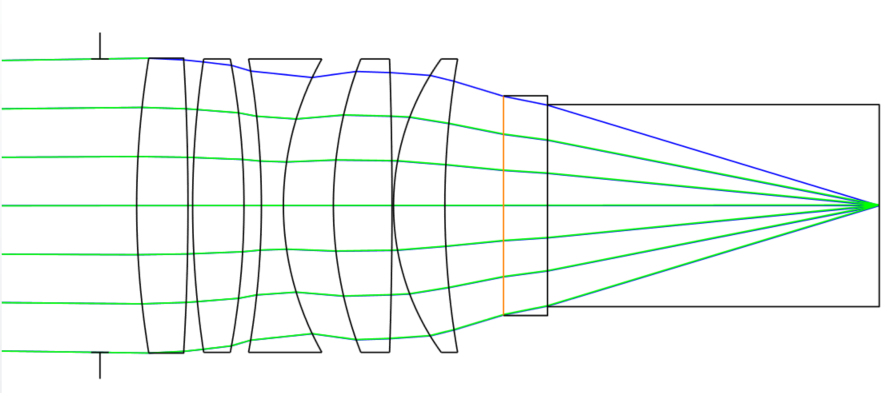
\includegraphics[width=\textwidth]{zeemaxobj}
%          \vspace{1em}
%          \caption{Zemax simulation of the objective. On the right, viewport and the vacuum chamber are also present.}
%          %\label{fig:three sin x}
%
%      \end{subfigure}
%         \caption{}
%       %  \label{fig:three graphs}
% \end{figure}
\begin{figure}
      \centering
          \centering
          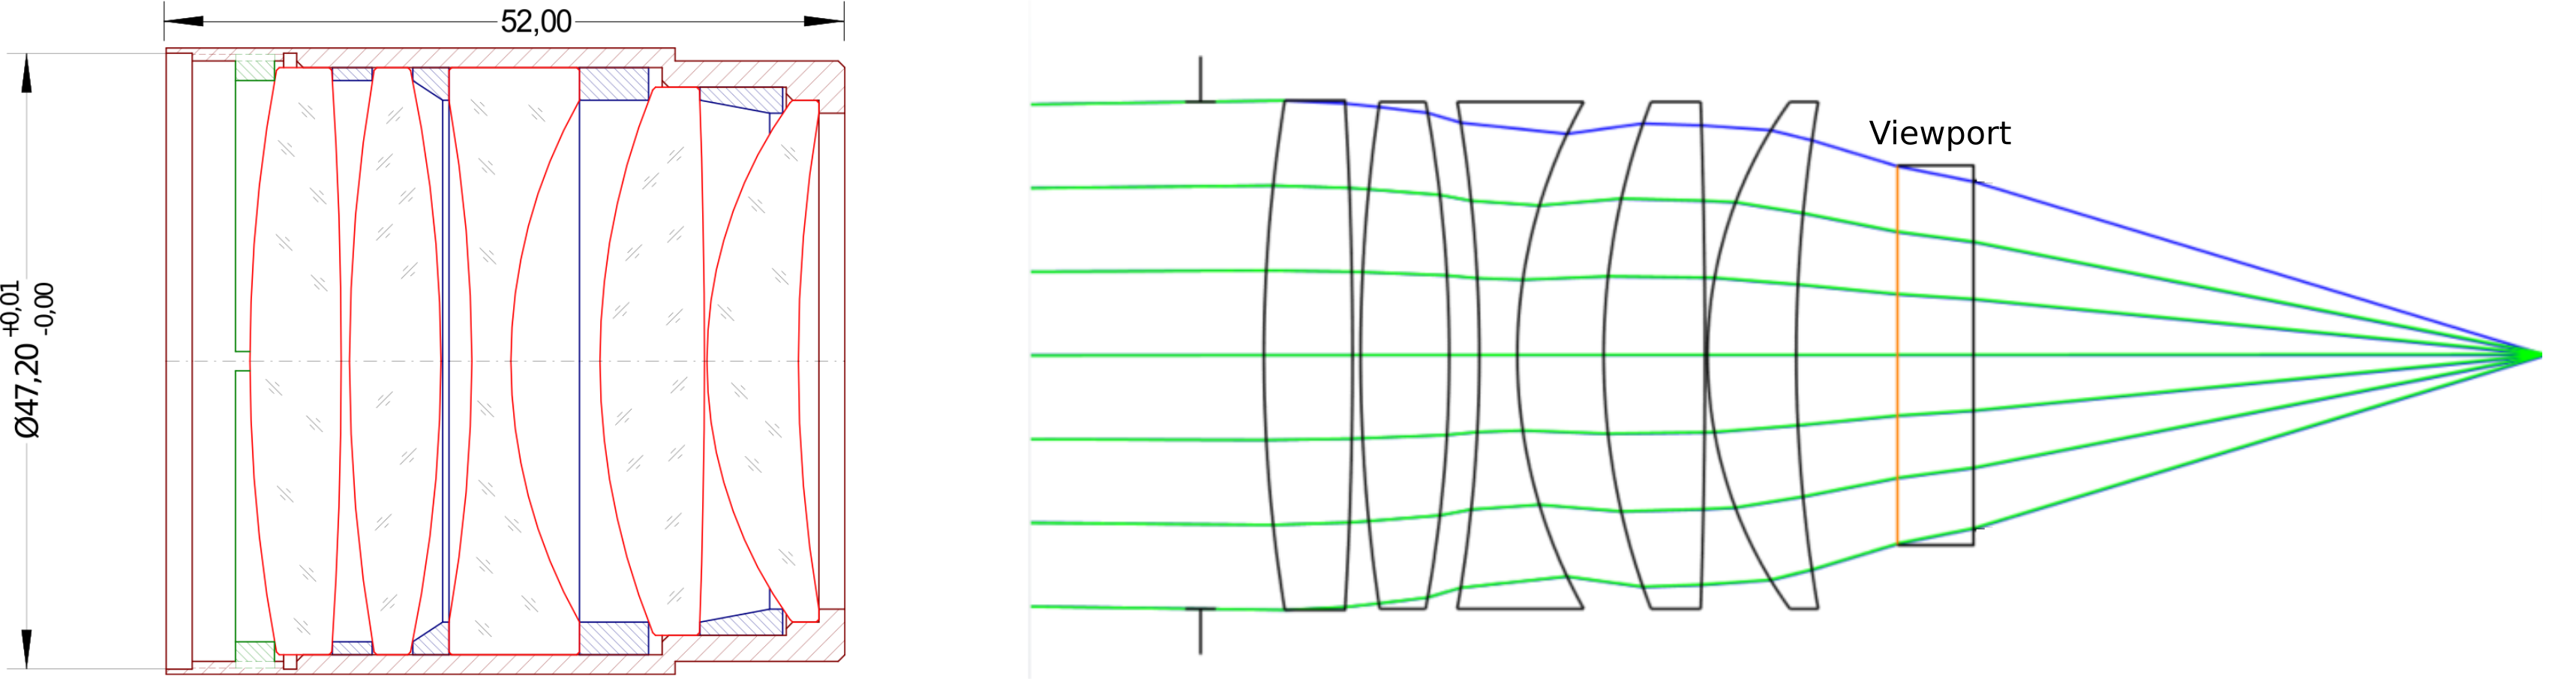
\includegraphics[width = \textwidth]{obj+zemaxpng}
           \caption{On the left, section of the custom objective made by Sill Optics, in red the 5 lenses are depicted, while the rest is the mechanical housing, given dimensions are in mm. On the right, Zemax simulation for 397 nm light: 5 lenses for the objective, a 6 mm viewport, and, after 38.6 mm of vacuum, the ions.}
          \label{objsection}
\end{figure}
The objective used to focus the light is a custom objective by Sill optics, Figure \ref{objsection} presents the model and a Zeemax simulation made by Sill Optics. This objective has different purposes: collecting 397 nm photons from ions, and imaging them onto a spot 1.5 meters away from the chamber; single-ion focusing with 729 nm light, taking incoming collimated 729 nm light and focusing onto an ion. The numerical aperture is NA = 0.289, thus effective focal length $f = 66.8$ mm. Furthermore, the objective was designed to take into consideration that the light after the objective has to go through a 6 mm fused silica viewport and a further 38.6 mm of vacuum before reaching the ions. The objective is mounted on a 3 dimensional manual translational stage to allow for imaging and addressing calibration.\par
The AOD is from Gooch \& Housego, model 4120-3, the datasheet is in Appendix \ref{sec:aoddata}. The crystal is Tellurium dioxide (TeO$_2$). The company specifies a central frequency of 120 MHz, with 50 MHz bandwidth, so the driving frequency ranges from 95 to 145 MHz with a maximum RF power of 0.3 W. Addressing spatial range of 30 mrad, i.e. angle of deflection $\pm 0.86^{\circ}$. In this bandwidth the diffraction efficiency should remain above 75 \% and have an average of 83 \%, further 3\% of light is lost due to insertion losses. The active aperture measures $3\times 3$ mm, and the polarization has to be horizontal when entering the AOD, while the specified output polarization is vertical.

\section{Design simulation}
I simulated the setup in Figure \ref{addressingsetup} with the software Zemax\footnote{Zemax OpticStudio is a commercial software based on ray tracing used for designing optical systems.}. The simulation had the purpose of assessing the performance of the setup and to find suitable lenses and their optimal locations. The simulation included: the four lenses, the objective, and the viewport. As there is no option to simulate an AOD, it was not taken into consideration, instead the simulation started at the output of the AOD as described below. Mirrors and beam splitters were not included in the simulation as their imperfections are not known.
\begin{figure}
\centering
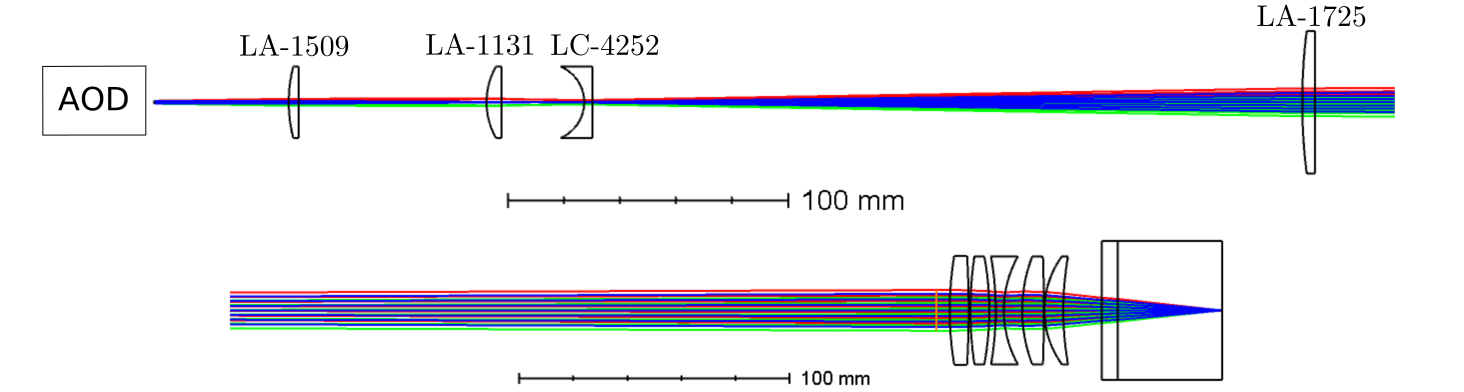
\includegraphics[width = \textwidth]{2levelszemax}
\caption{Zemax simulation of the setup. Rays propagate from left to right starting from top left. Simulation layout has been separated in two for displaying purposes. In the top part, the four lenses are depicted, the rays continue in the bottom part where the objective and image plane are located. Different colors indicate different beams emerging from the AOD at different angles, rays with the same color belong to the same beam. The blue one is the central beam emerging from the AOD with a 0$^\circ$ angle, the red and the green beams emerge respectively with $\pm0.86^\circ$.}
\label{zemaxview}
\end{figure}
The simulation starts by specifying the input fields, representing the physical light beam at the output facet of the AOD. To account for the ability to change the output angle from the AOD, three different fields have been simulated. One is along the optical axis, while the other two are angled corresponding to the extrema of the AOD bandwidth, so $\pm0.86^{\circ}$. The propagation of these fields represents three different situations of beam direction and should also give an idea of the behavior in between the extrema. Next, the four lenses of the setup were inserted in Zemax, initially with variable radii, thicknesses and separations. Initial positions and lens focal lengths were set according to geometrical boundaries given by physical constraints on the optical table where the setup had to be built. In fact, the  setup has to be built inside the mu-metal chamber surrounding the ion-trap experiment. The Zemax file of the objective came from the company which designed it\footnote{There are currently 2 versions of the files. Both contains the same objective but with slightly different composite lenses. Effectively, the difference in the simulation is the focal length: 54 mm and 52 mm. However, by adjusting the distance between the objective and the viewport (which is unknown at the mm level in the experiment), this difference is compensated and their performance is identical. In the simulation the 54 mm version is used.} and was simply imported in the project. After the objective the 6 mm viewport glass was included and then vacuum for 38.6 mm, which is the expected distance between the outer facet of the glass and the ion axis. The image plane was therefore set 38.6 mm after the viewport. In the experiment, the distance between the objective and the viewport could not be measured (the objective lies inside an inverted viewport and there is no access space for distance measurement at the mm level). However, this distance was inferred from a Zemax simulation of the imaging path, assuming that the ions focus on the camera 1.5 m away, we determined a space between the viewport and the objective of 14 mm.\par
The simulation was carried out with the Zemax tool Physical Optics Propagation (POP). POP works by propagating a wavefront represented by an array of discrete points\footnote{grid of 30.6$\times$30.6 mm, sampled with $256\times256$ points.}. The array is propagated through every optical component and free space. This method can be used to simulate Gaussian beams as well as wave phenomena such as diffraction and aberrations. The initial value given to the propagator was the waist of the collimated beam out of the AOD. Since the beam going to the AOD comes from a fiber collimator, the value specified was taken from the datasheet of the fiber collimator, namely Sch\"after + Kirchhoff 60FC-M12-33 \cite{fibercollimator}, as 1.07 mm.
\begin{figure}
     \centering
     \centering
     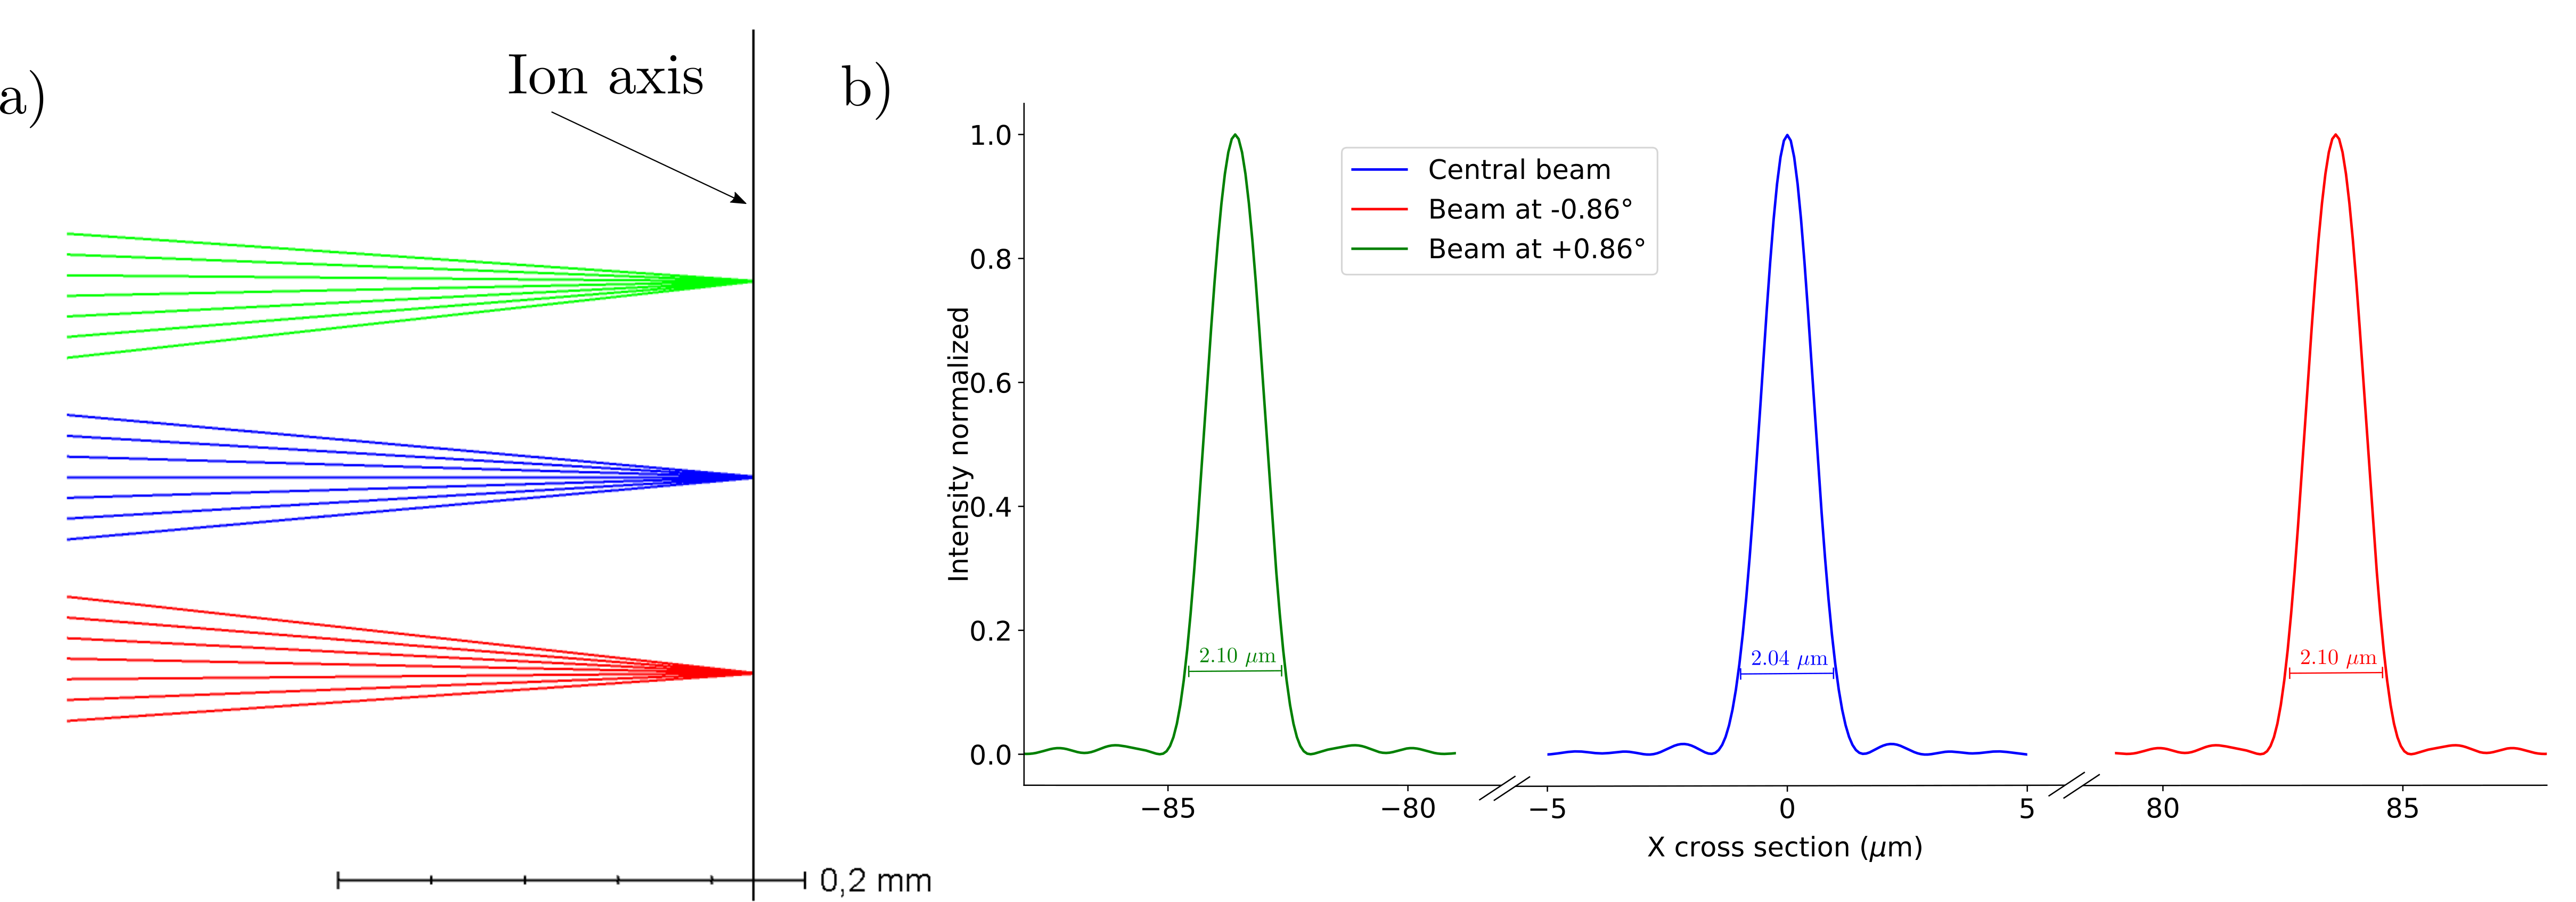
\includegraphics[width=1\textwidth]{img/range_plus_3beams}
     \caption{Zemax simulation at the image plane, where the ions are. a) Addressing range from Zemax simulation, the three beams emerge from the AOD at different angles. The full addressing range here displayed is 168 $\mu$m. b) Physical Optics Propagation of the three Gaussian beams with angles of $0,\pm0.86^\circ$, and waist at AOD of 1.07 mm. Displayed is the $x$ cross section at the ion axis. Beam diameters (13.5\%) are also displayed, the central beam at 2.04 $\mu$m is slightly narrower with respect to the outer ones $2.10$ $\mu$m.}
     \label{zemaxrange}
\end{figure}
The first step of the simulation work was to find the appropriate lenses to build the setup. The thicknesses and the radii of curvature were optimized trying to achieve the smallest focus spot while maintaining the desired addressing range. The lenses were found with the Zemax tool \emph{Stock Lens Matching}. Basically, the tool compares the simulated lenses with those in a catalogue from different companies and finds the closest match. We opted to rely on the provider Thorlabs, so the search was limited to this company. Found lenses were in order from left to right LA-1509, LA-1131, LC-4252, and LA-1725 and can be seen in Figure \ref{zemaxview}. Once the desired lenses were found, their Zemax files provided by the company were imported in the project.\par
The second step was to optimize the lenses position's always trying to keep the focus spot as small as possible, and the desired addressing rage of 150-200 $\mu$m. This was done using the optimizing tools of Zemax and the merit function. The software can perform multivariate analysis and minimize the focus spot depending on all the assigned variables, which in this case were the distances between the lenses. The final results, for the lens setup shown in figure \ref{addressingsetup}, is presented in Figure \ref{zemaxrange}, the addressing range is 168 $\mu$m limited by the bandwidth of the AOD from the specification sheet. The waist of the central beam is $1.02\,\mu$m, and beam profiles at the border of the addressing range are $3\%$ broader, with a waist of $1.05$ $\mu$m.\par
Another important parameter for the performance of the setup is the addressing error. Qualitatively speaking, in the case of the beam focused on one ion, the addressing error is caused by the light interacting with the neighbour ions. It can be a particular problem in the case of aberrations that produce bumps on the side of the main Gaussian peak. In the case of a diffraction limited system, the profile of the beam is a sinc function that has more local maxima around the central peak. To estimate the addressing error in a simulation, we consider two ions 5.6 microns apart, centered on the optic axis of the addressing system, the respective addressing beams have been simulated. In Figure \ref{zemaxaddrerror.png} the intensity profile and the electric field are plotted. The addressing error is different for different physical process, in the case of AC Stark shift, as the experiment discussed in \ref{sec:expqubit}, the shift is proportional to the intensity, so the addressing error is calculated as $I_1(x_2)/I_1(x_1) \simeq 10^{-4}$, where $I_{1}$ is the intensity profile of the beam focused on ion 1, and $x_1,x_2$ are respectively the position of ion 1 and ion 2. In the case of the cavity mediated Raman process, as in the experiment discussed in Section \ref{sec:expphoton}, the strength of the process is proportional to the Rabi frequency, i.e. the electric field. Therefore, the addressing error is given as $\sqrt{I_1(x_2)/I_1(x_1)} \simeq 10^{-2}$.\par
 \begin{figure}
 \centering
 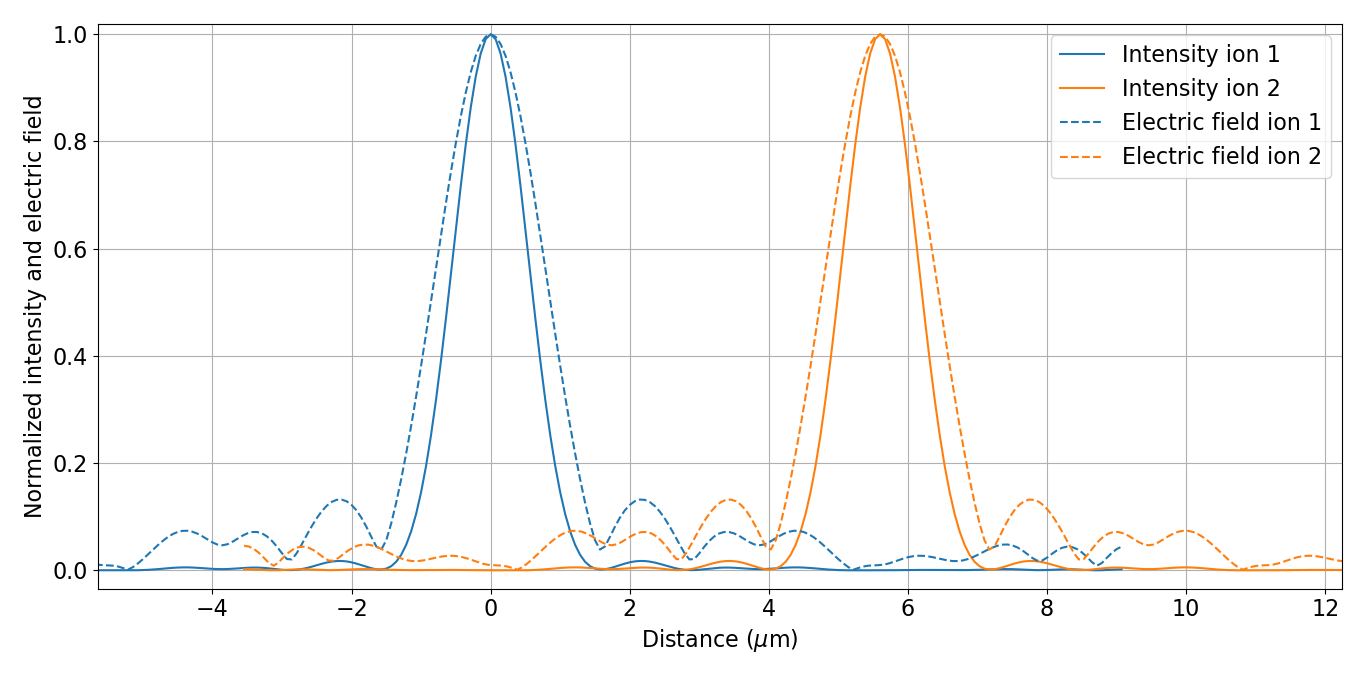
\includegraphics[width = .9\textwidth]{zemaxaddrerror3}
 \caption{Zemax simulating of the beam focused in two different places separated by 5.6 $\mu$m corresponding to the theoretical equilibrium positions of two ions with axial center of mass frequency of 1 MHz. Addressing error for AC Stark shift is calculated as the ratio of intensities at ion positions: $I_1(x_2)/I_1(x_1) \simeq 10^{-4}$. For Raman transition, the ratio of electric fields is taken: $\sqrt{I_1(x_2)/I_1(x_1)} \simeq 10^{-2}$.}
 \label{zemaxaddrerror.png}
 \end{figure}
Another aspect that was simulated is the beam profile inside our ion trap system. Optical access to the trap is limited and a tightly focused beam also has correspondingly a large divergence, which could lead to clipping on the trap's blades or compensation electrodes, scattering light all around the trap. In Figure \ref{lossesplot} the top view of the trap is plotted, here we included the three pairs of compensation electrodes, the RF blades, and the cavity mirrors. The blue line represents the radius $W(z)$ from Equation \ref{waistprofile} of the addressing beam in the case of a waist $W_0$ of 1 $\mu$m. To determine the fraction of power lost due to clipping on the compensation electrodes, we can calculated the transmitted power through the top electrodes:
\begin{equation}
P_{t} = \int_{-\infty}^{\infty}\text{d}y \int_{-x_c/2}^{x_c/2}\text{d}x P(x,y,z),
\end{equation}
where $P(z)$ is the power of the Gaussian beam, and $x_c$ is the horizontal position of the compensation electrode. The integral can be computed numerically at position $z$ of the electrodes. The result is plotted in Figure \ref{lossesplot}, where the lost power $1-P_{t}$ is plotted as a function of the waist $W_0$. At the expected waist of $1.02\,\mu$m, the power lost is less than 1\%, i.e. for 2 $\mu$W AOD input power, after considering all the losses in the setup, it means losing less than a nW. The previous calculation holds only if the beam is perpendicular to the $x$ direction so it is important to align it carefully. Note that the ion trap was designed without an electrode pair on one side, to avoid back reflections of the addressing beam, into the direction of the imaging apparatus.\par
\begin{figure}
       \centering
         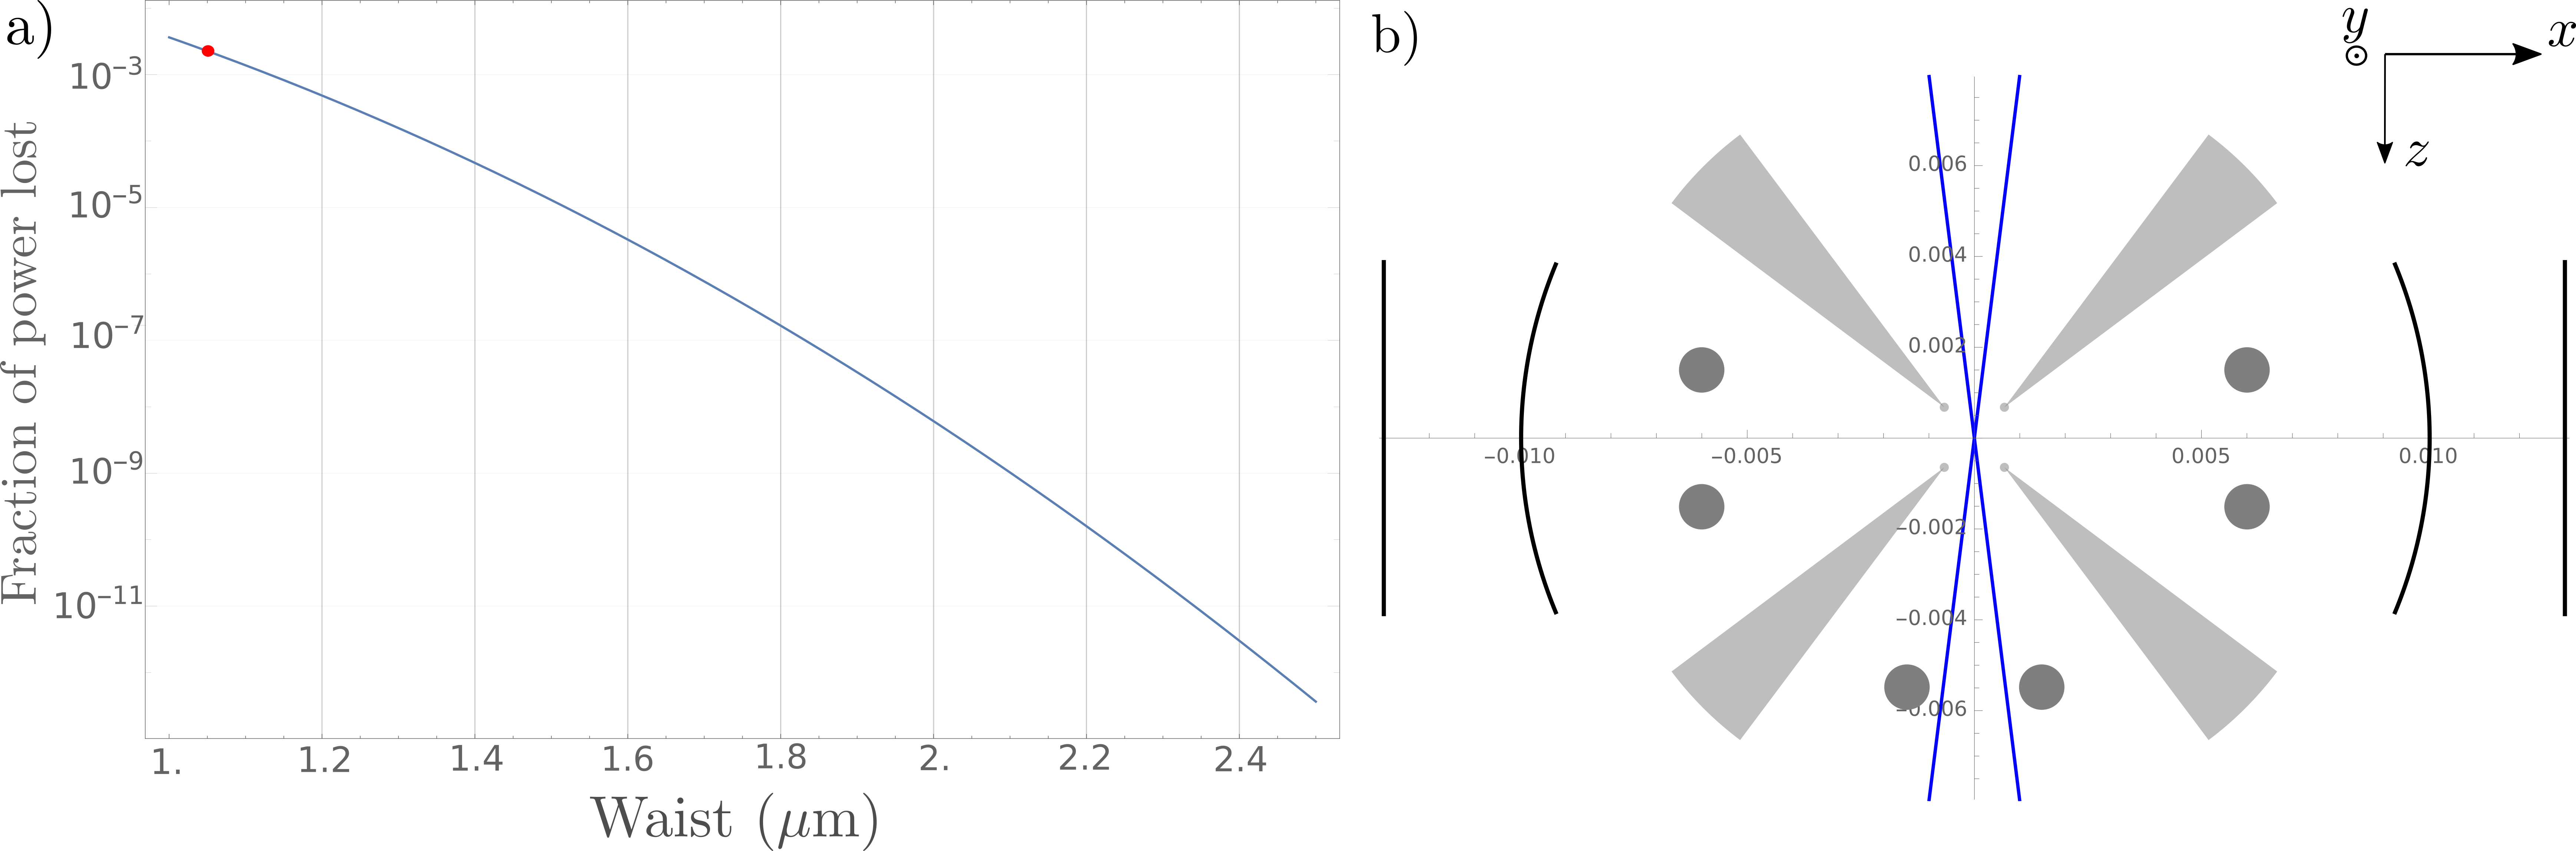
\includegraphics[width=\textwidth]{powerlost_plus_diagram2}
         \caption{a) Fraction of power lost due to clipping on the compensation electrodes as a function of the beam waist when focused on ion. Red point represents the waist $1.02\,\mu$m, obtained from the simulation. b) Top view of the trap and addressing beam. Grey circles are the compensation electrodes, blue is the radius $1/e^2$ of the beam focused on the ions with waist of 1.02 $\mu$m, while the black arches represent the mirrors of the cavity. All units are in meters.}
         \label{lossesplot}
 \end{figure}
To conclude this section, we discuss some aspects of the design. Waist and addressing range were the two key aspects. In the last stage of the simulation, the distances between the lenses were optimized, and their position is a compromise between waist and addressing range, it is possible therefore to sacrifice one to improve the other. We found that the addressing range can be broadened by moving the beam expander closer to the objective, simulations yielded an addressing range of 180 $\mu$m for a distance between objective and lens LA-1725 of 622 mm, in this case the distance between this lens and the diverging one is 262 mm to keep the focus at the same position. In this configuration a greater addressing range is achieved, but the waist at the ions is 1.10 $\mu$m, broader then the 1.02 $\mu$m presented in this section. In the simulation, an attempt to decrease addressing range for a smaller waist by moving the beam expander farther away from the objective fails, the addressing range is reduced, but the waist does not significantly change as the full diameter of the objective is being used. Moreover in this case, the aberrations, already noticeable in Figure \ref{zemaxaddrerror.png}, get worse, the small bumps on the side of the main peak increase in height. This could suggest that the system is diffraction limited at the entrance of the objective, the bumps are in fact attributable to a Airy pattern commonly associated with diffraction limited system \cite{dlimited}.
\section{Physical implementation}
\label{design4}
Once the simulation gave satisfactory results, a test setup was built. The idea of building first a test setup on a different optical table from the main experiment was to check if the system was working as intended, and asses its performance. Due to physical access problems in the final system there is no space to place a beam profiler, or a polarimeter, and after the objective there is no access to the vacuum and the trap. While on another table everything could be checked and tested. The results of the measurements obtained on this test setup are presented in Chapter \ref{ch:results}.\par
Afterwards, the system was moved and implemented on the optical table containing the ion trap. For the initial alignment, a counter propagating red beam was sent in the opposite direction: starting from the front of the chamber, through the ions, and through to the objective and back through the addressing path. Since the lenses of the addressing are antireflection coated for 393 nm, the reflection of the red beam was visible and it was possible to align the components such that the beam passed approximately through the center and perpendicular to the surfaces. Calibration was also done with ions and the beam position was indirectly observed on the camera via the excited fluorescence of the ions. A string of ions was used as a probe by constantly imaging the ions with 397 nm (illuminating the entire string equally) and 393 nm (illuminating ideally a single ion) light on the camera. The 393 nm laser drives the transition $\text{S}_{1/2}\leftrightarrow \text{P}_{3/2}$. From $\text{P}_{3/2}$ the electron has two other decay channels, $\text{D}_{3/2},$ and $\text{D}_{5/2}$, which means that the electron will eventually end up in one of these two states. Repumping with 854 nm and 866 nm light the transitions $\text{D}_{5/2}\to \text{P}_{3/2}$, and $\text{D}_{3/2}\to \text{P}_{1/2}$ avoids this problem and brings the electron back to the fluorescence cycle. To observe where the addressed 393 nm beam is, we send pulses of 854 nm light
such that when the 854 nm light is off the ions addressed by the 393 nm laser become dark after decaying from $\text{P}_{3/2}\to  \text{D}_{5/2}$. The ions become bright again when a new pulse of 854 nm light is sent, therefore if the pulse rate is slow enough it is possible to see the addressed ions as blinking on the CCD camera. This process was used for initial alignment of the addressing beam focus and direction on the ion string. Once done, the next stage is to directly measure and optimize the AC stark shifts, as presented later in section \ref{sec:singlequbitmanipulation}.\par
A photo of the installed system is in Figure \ref{photosetup}. Here, the collimating lens is mounted on a 3D manual screw-gauge translation stage for fine tuning calibration position of the focus w.r.t. the ion string. Manual screws were later replaced with remote controlled ones from Newport, model PZA12 so that beam alignment is possible without opening the mu-metal enclosure. The AOD is placed on a rotation mount that allows to tilt it in two directions. One direction was used to find the Bragg angle of the AOD to achieve maximum diffraction efficiency, the other can be used to tilt the axis over which the AOD sweeps to compensate for an ion string which is not exactly parallel to the AOD sweeping direction.

\begin{figure}
\centering
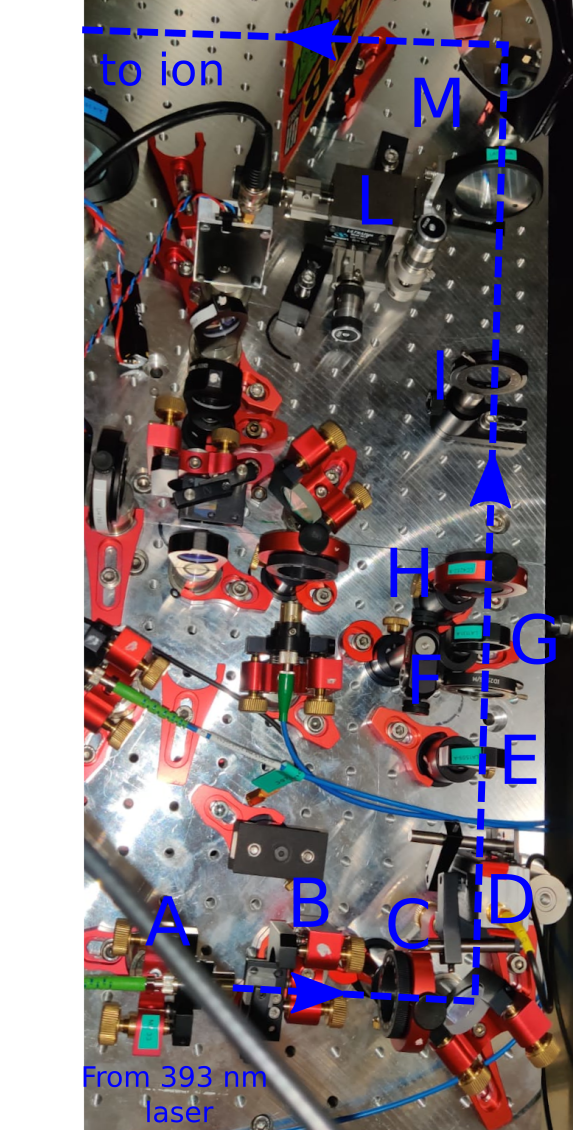
\includegraphics[scale = 1.3]{photosetupnice_withlabels2.png}
\caption{Photo of the single-ion addressed optical setup. The blue dashed line is the beam path starting from bottom left at the fiber collimator, all the way to the top where a mirror deflects the beam and send it to the 90:10 beam splitter (Figure \ref{addressingsetup}). The following elements are visible: (A) Fiber collimator 60FC-M12-33 (B) Polarizing beam splitter (C) $\lambda/2$ (D) AOD (E) Lens LA-1059 (F) Iris to block 0th order (G) Lens LA-1131 (H) Diverging lens LA-4252 (I) Iris (L) Lens LA-1725 on the 3D manual screw-gauge translation stage (M) Mirror. }
\label{photosetup}
\end{figure}
